% Intended LaTeX compiler: pdflatex
\documentclass[presentation]{beamer}
\usepackage[utf8]{inputenc}
\usepackage[T1]{fontenc}
\usepackage{graphicx}
\usepackage{longtable}
\usepackage{wrapfig}
\usepackage{rotating}
\usepackage[normalem]{ulem}
\usepackage{amsmath}
\usepackage{amssymb}
\usepackage{capt-of}
\usepackage{hyperref}
\usetheme{Montpellier}
\AtBeginSection[]{\begin{frame} \vfill \centering \begin{beamercolorbox}[sep=8pt,center,shadow=true,rounded=true]{title} \usebeamerfont{title}\insertsectionhead\par \end{beamercolorbox} \vfill \end{frame}}
\usetheme{default}
\author{Jan Boone}
\date{Work in Progress}
\title{Health effects of OOP}
\hypersetup{
 pdfauthor={Jan Boone},
 pdftitle={Health effects of OOP},
 pdfkeywords={},
 pdfsubject={},
 pdfcreator={Emacs 28.2 (Org mode 9.5.4)}, 
 pdflang={English}}
\begin{document}

\maketitle
\begin{frame}{Outline}
\setcounter{tocdepth}{1}
\tableofcontents
\end{frame}




\section*{Introduction}
\label{sec:orgafef9d2}

\begin{frame}[label={sec:orgfc622fb}]{Health insurance}
\begin{itemize}
\item healthcare costs increase in all developed countries
\item health insurance can cause moral hazard
\item oop payments is one way to mitigate this
\item if a deductible increase reduces expenditure, we view this as welfare enhancing
\begin{itemize}
\item trade off: risk aversion
\end{itemize}
\item what if oop cause people to postpone \emph{valuable} treatments?
\item can we identify this effect across countries?
\end{itemize}
\end{frame}

\begin{frame}[label={sec:org8bc88cc}]{Health effects}
\begin{itemize}
\item postponing/forgoing valuable care has health effects
\item measuring health effects is not easy
\item we use mortality per NUTS 2 region/year/age/gender in European countries
\item fixed effects to control for non-observed variables
\end{itemize}
\end{frame}

\begin{frame}[label={sec:orgc0e0b0f},fragile]{Insurance generosity}
 \begin{itemize}
\item comparing insurance generosity across countries is not straightforward
\item how to compare a system with high deductible but low coinsurance rate?
\item we use \texttt{OOP}: \% oop in total health expenditure
\item high oop is especially problematic for people on low income
\item they could forgo valuable treatment if it is expensive
\item if this mechanism exists: higher mortality in regions where \texttt{OOP} \(\times\) \texttt{Poverty} is high
\end{itemize}
\end{frame}

\begin{frame}[label={sec:org954a2fc}]{NUTS 2 regions in Europe}
\begin{center}
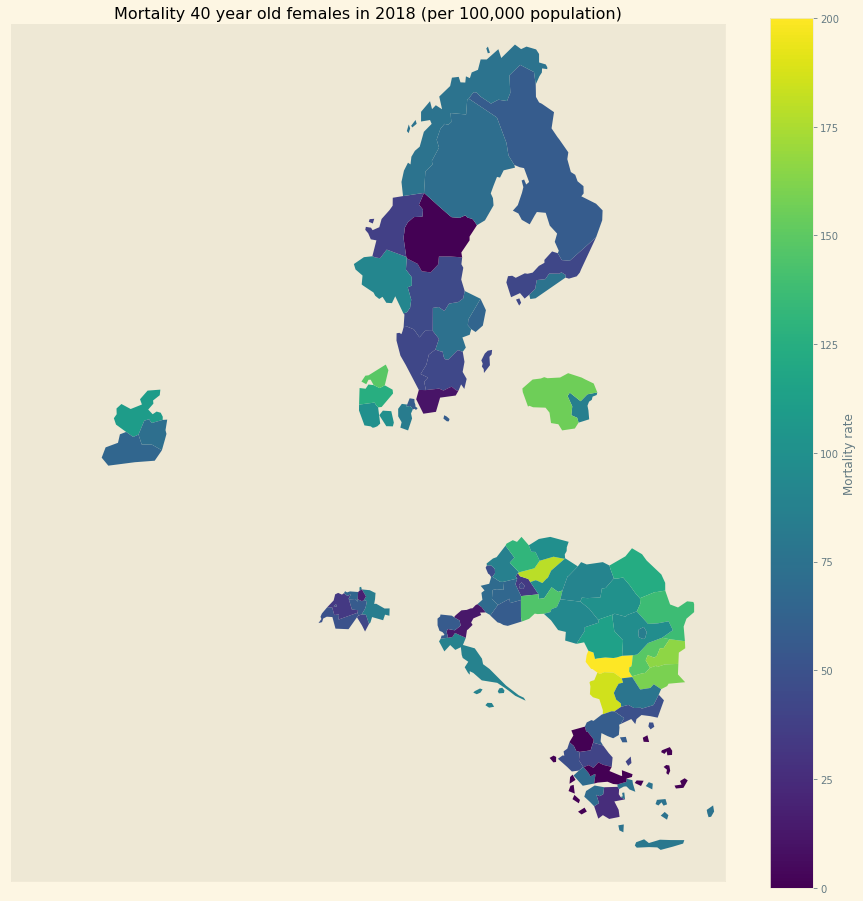
\includegraphics[width=.6\linewidth]{./figures/Europe_mortality_40_F_2018.png}
\label{fig:EUmap}
\end{center}
\end{frame}

\begin{frame}[label={sec:org58d3245}]{summary}
\begin{center}
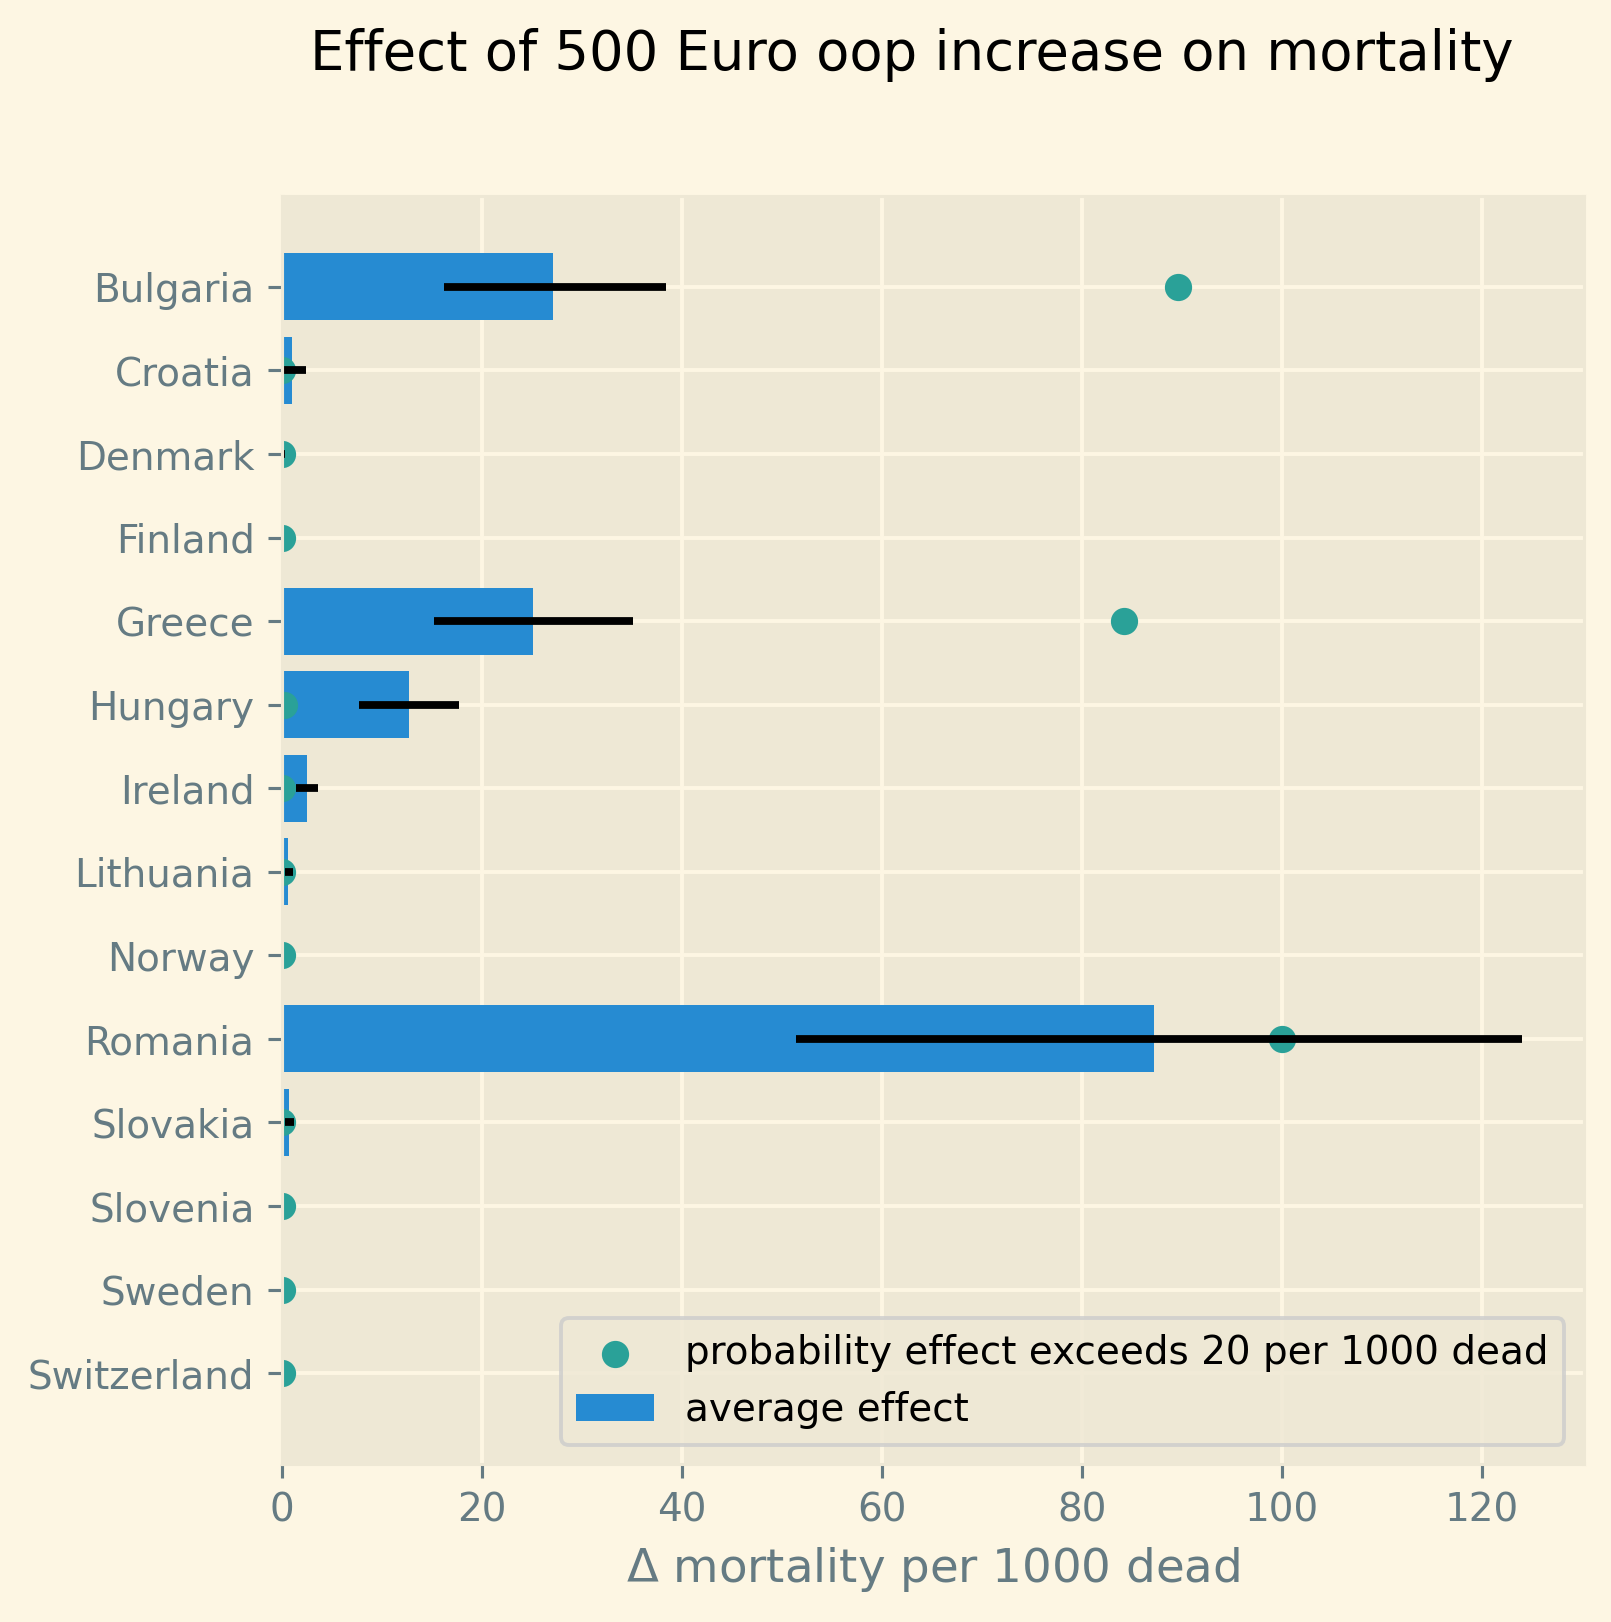
\includegraphics[width=0.6\linewidth]{./figures/change_mortality_countries_baseline.png}
\label{fig:SummaryFigure}
\end{center}
\end{frame}



\begin{frame}[label={sec:org56a2b53}]{Literature: individual level data}
\begin{itemize}
\item recent literature on relation oop and mortality
\item US individual level data
\item e.g. Miller et al. (2021) on Medicaid eligibility expansion:
\begin{itemize}
\item introduced in different states at different times
\end{itemize}
\item Chandra et al. (2021) Medicare part D prescription drug coverage
\begin{itemize}
\item enrollment month
\end{itemize}
\item behavioral hazard: Baicker et al. (2015)
\end{itemize}
\end{frame}

\begin{frame}[label={sec:orgef8585b},fragile]{This paper}
 \begin{itemize}
\item European regional data
\item more broad brush: cannot capture effect of 1\% increase in deductible
\item compare health insurance systems that are more/less generous
\item more variation in \texttt{OOP} than with Dutch individual level data
\item European health insurance more homogeneous across regions in a country
\end{itemize}
\end{frame}

\section*{Two equations to estimate}
\label{sec:orgba26dfa}

\begin{frame}[label={sec:orgb44f304},fragile]{theory}
 \begin{itemize}
\item using a theoretical model we derive two equations to estimate:
\begin{itemize}
\item probability of death as a function of \texttt{Unmet} medical needs
\item probability that someone forgoes treatment because it is too expensive as a function of \texttt{OOP} and \texttt{Poverty}
\end{itemize}
\end{itemize}
\end{frame}

\begin{frame}[label={sec:orgc03c79b}]{Number of deaths}
\begin{itemize}
\item per age, gender, year, nuts 2 region
\item \(k\) deaths out of \(n\) population: \(\binom{n}{k} m^{k}(1-m)^{n-k}\)
\end{itemize}
$$
m_{ga2t} = \frac{e^{\beta_{ag}}}{1+e^{\beta_{ag}}} e^{\left( \mu_2 + \gamma \ln \left(\frac{m_{a-1,g,2,t-1}}{\bar{m}_{a-1,g}}\right)+ \beta_{poverty}\text{Poverty}_{2t} + \beta_{unmet}\text{Unmet}_{2t}\right)}
$$
\end{frame}

\begin{frame}[label={sec:org964dcb9}]{Too expensive}
\begin{itemize}
\item one motivation for unmet medical needs is that treatment is too expensive
\item fraction of people in a region indicating that they postponed/forgone treatment because it was too expensive:
\end{itemize}
$$
\text{TooExp}_{2t} = b_{0,2} + b_{0,t} + \text{OOP}_{ct} \bar{x}_{ct} \left(  b_{oop,c} + b_{interaction,c} \text{Poverty}_{2t} \right)
$$
\begin{itemize}
\item equation is derived by varying co-insurance and deductible
\end{itemize}
\end{frame}


\begin{frame}[label={sec:org7aa6fc2},fragile]{Relation \texttt{OOP} and \texttt{TooExp}}
 \begin{center}
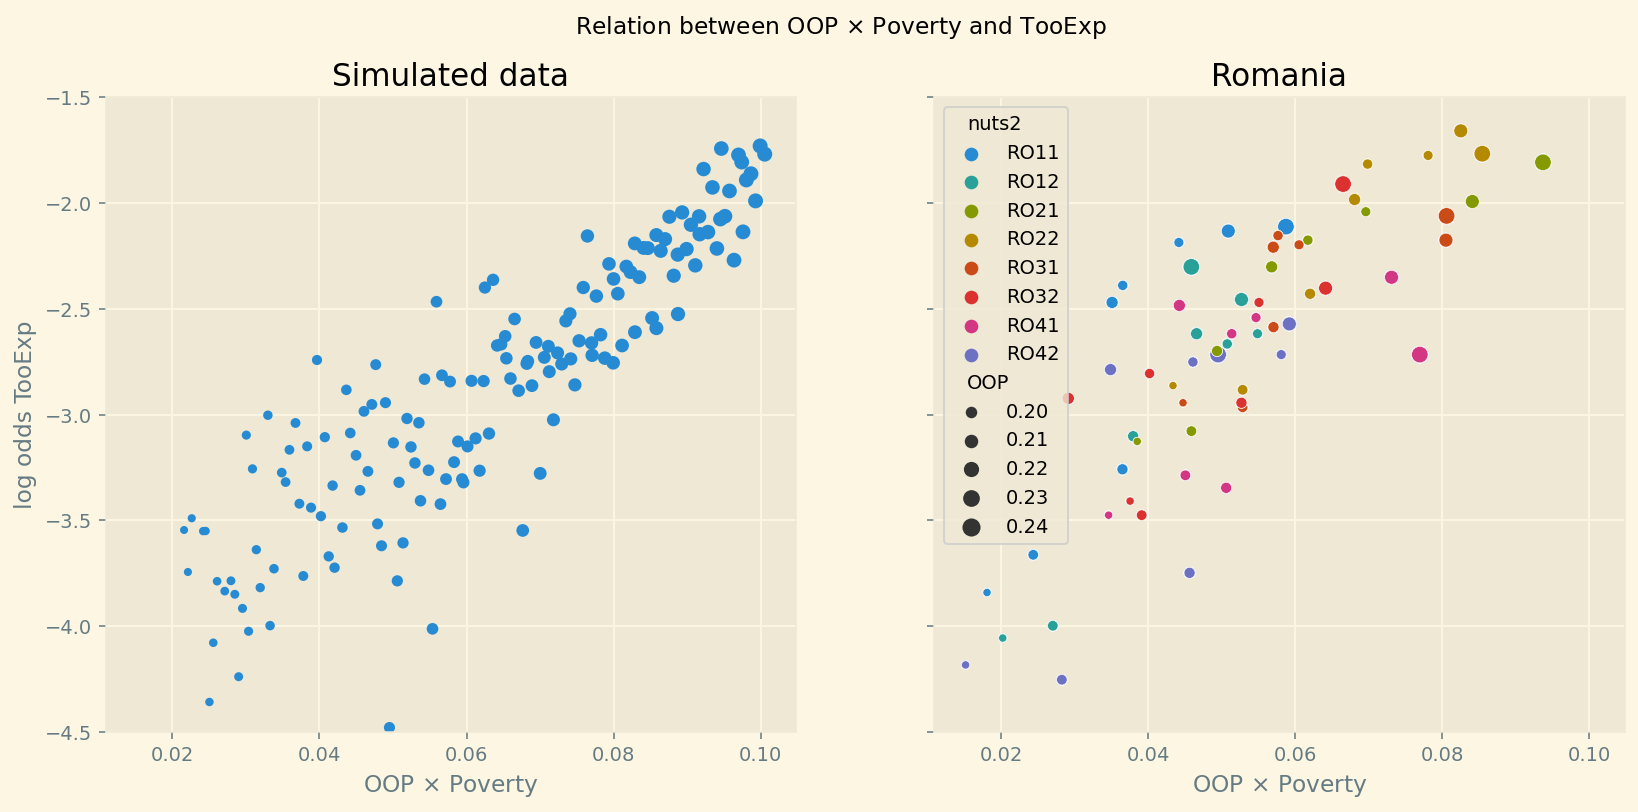
\includegraphics[width=.9\linewidth]{./figures/Parametric3.png}
\label{fig:Parametric}
\end{center}
\end{frame}

\section*{Data}
\label{sec:org93fd4a2}

\begin{frame}[label={sec:orgbf83a76}]{Eurostat data: 2009-2019; ages 35-85}
\begin{table}[htbp]
\caption{\label{tab:summary}Summary statistics main variables}
\centering
\begin{tabular}{lrrr}
 & count & mean & std\\
\hline
population & 52612.00 & 7491.28 & 4805.28\\
deaths & 52612.00 & 103.19 & 126.49\\
deprivation & 52612.00 & 11.23 & 12.78\\
too exp. & 52612.00 & 2.00 & 3.09\\
unmet & 52612.00 & 4.93 & 3.73\\
out-of-pocket & 52612.00 & 22.03 & 8.88\\
expend. per head & 52612.00 & 3379.56 & 2688.57\\
\end{tabular}
\end{table}
\end{frame}




\section*{Estimation}
\label{sec:org76e595d}

\begin{frame}[label={sec:org019dc2f}]{Estimation technique}
\begin{itemize}
\item Bayesian analysis: are we 95\% sure that the following chain of effects is present:
\begin{itemize}
\item higher oop leads to higher unmet needs in areas with high poverty
\item which then leads to higher mortality
\end{itemize}
\end{itemize}
\end{frame}

\section*{Results}
\label{sec:org31a59a0}

\begin{frame}[label={sec:org7f94455}]{Fit}
\begin{figure}[htbp]
\centering
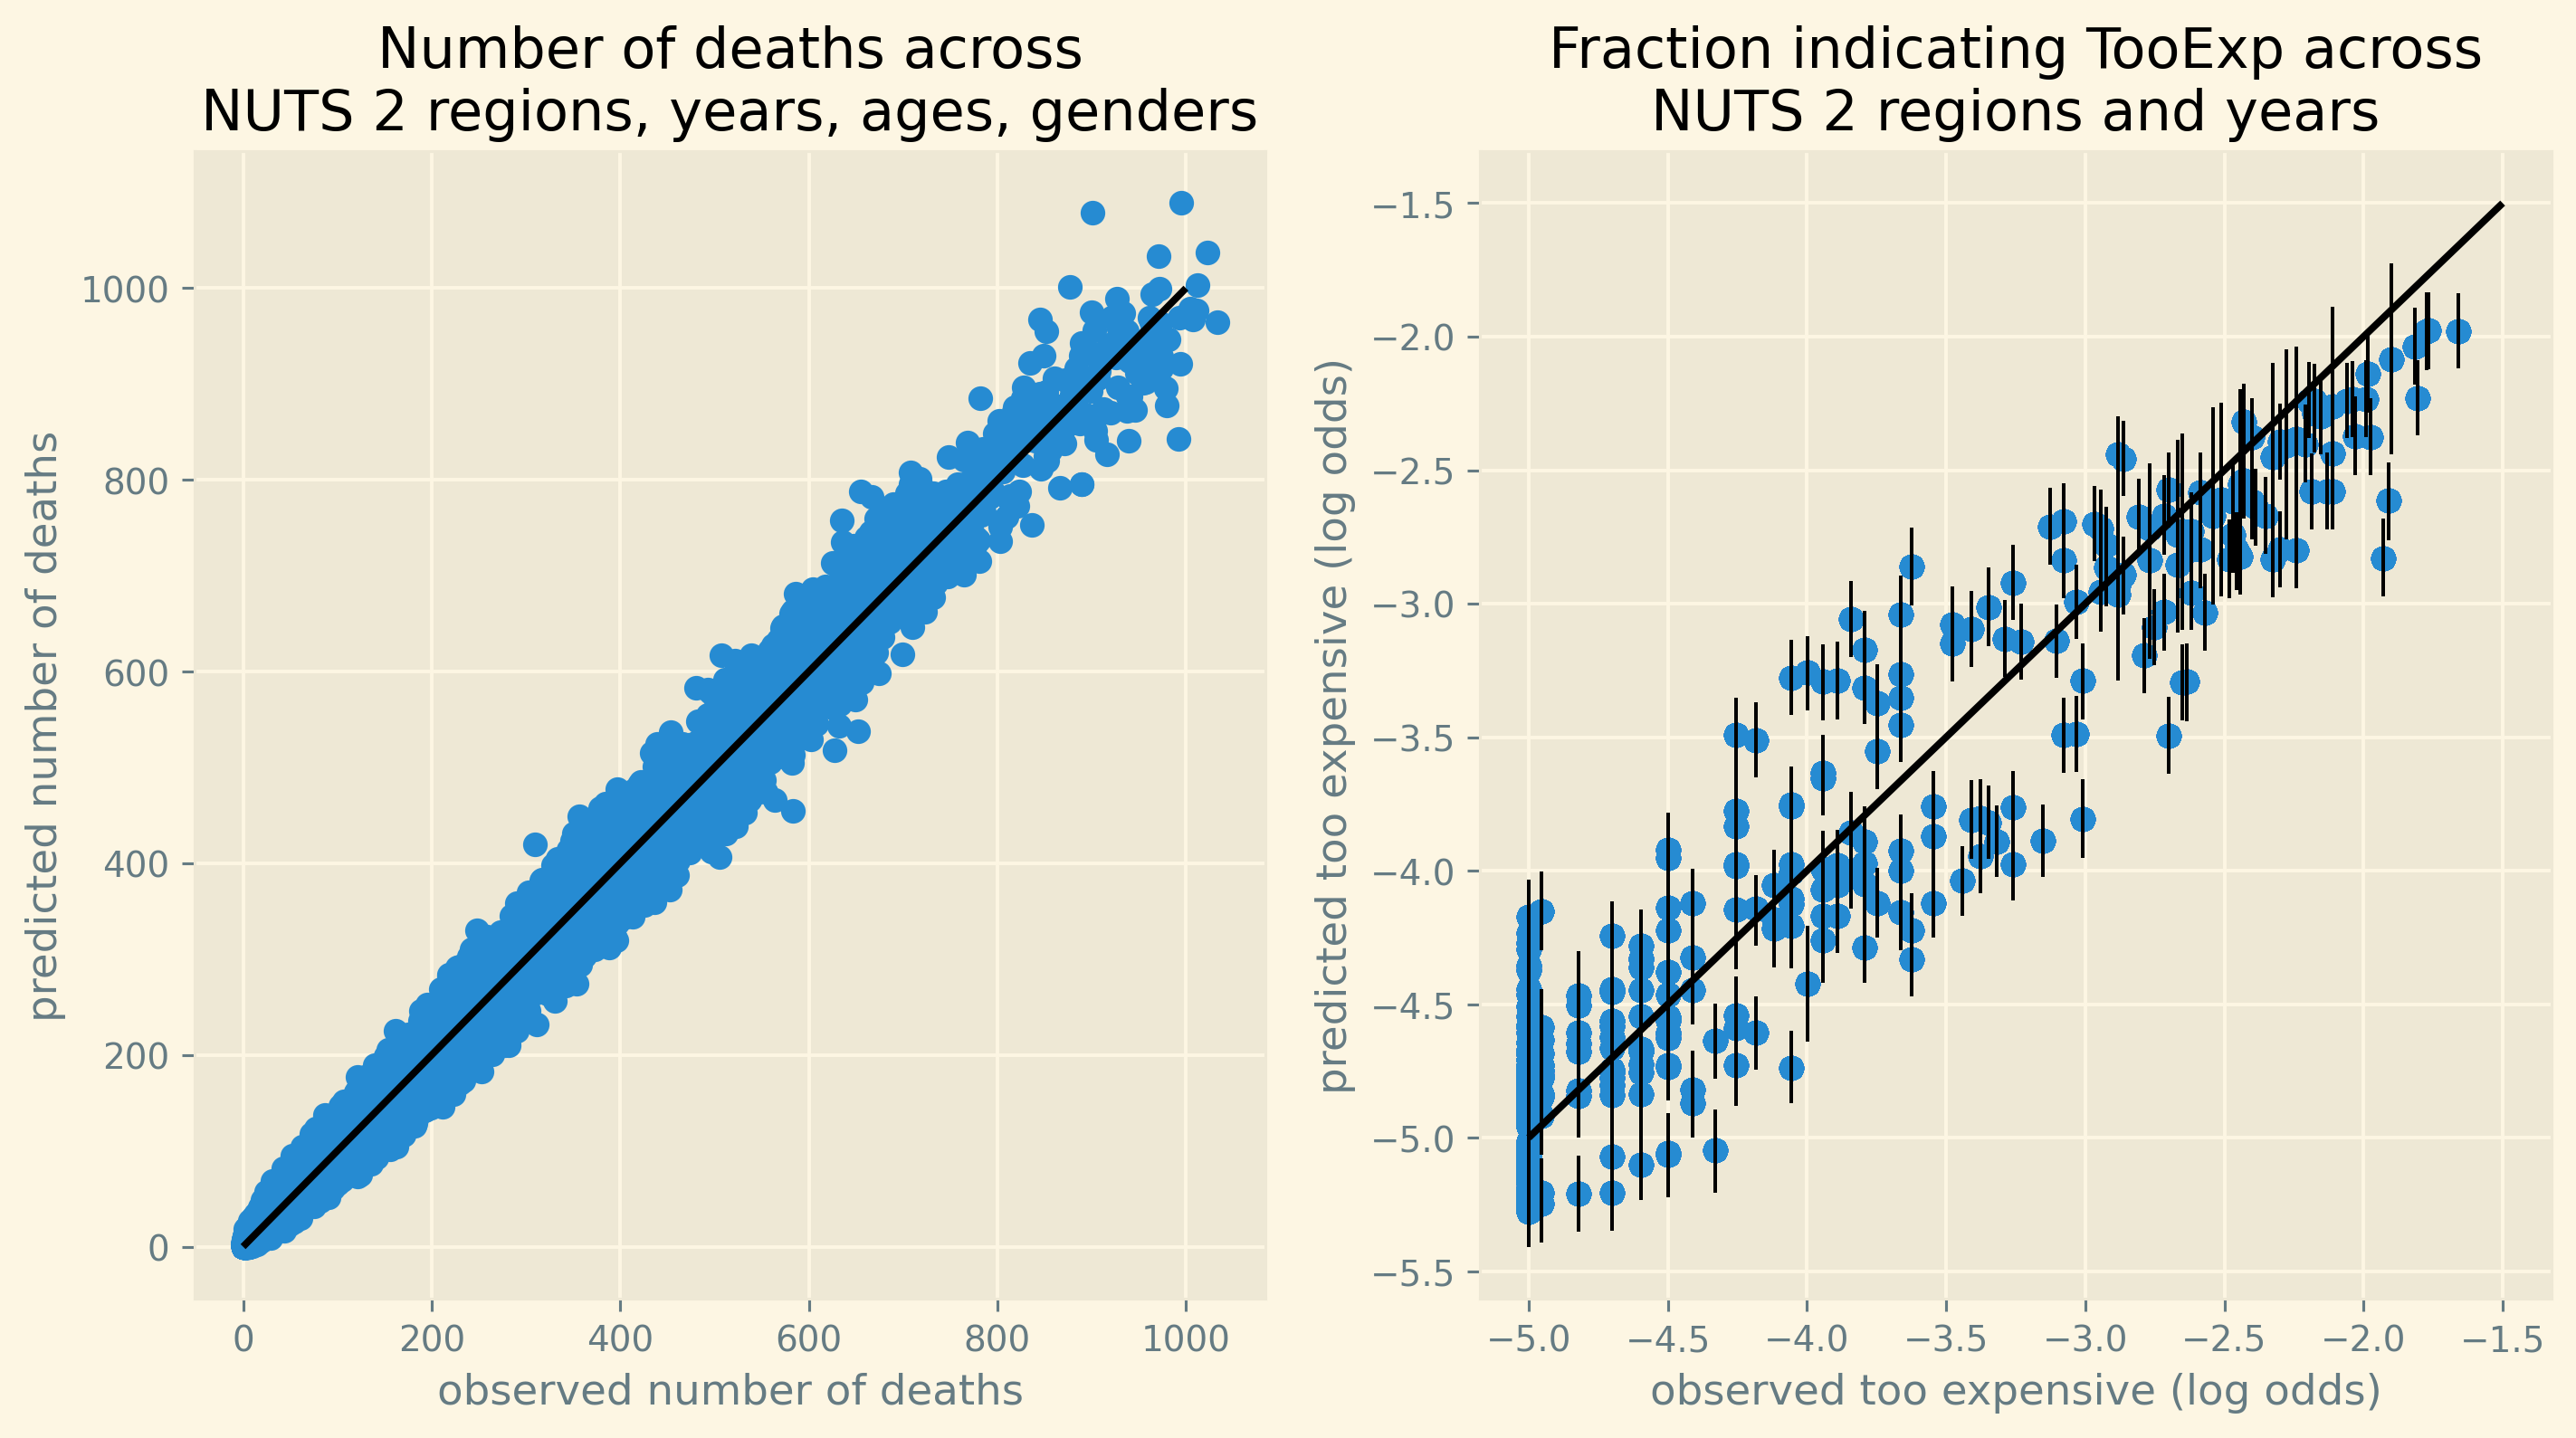
\includegraphics[width=.9\linewidth]{./figures/fit_baseline_model.png}
\caption{\label{fig:ModelFit}Fit of estimated and observed mortality across all observations.}
\end{figure}
\end{frame}


\begin{frame}[label={sec:org0b50dec}]{NUTS 2 region per country}
\begin{table}[htbp]
\caption{\label{tab:region_per_country}Region per country with highest fraction of material deprivation}
\centering
\begin{tabular}{llrr}
region & country & deprivation & too expensive\\
\hline
BG33 & Bulgaria & 0.40 & 0.08\\
HR04 & Croatia & 0.13 & 0.01\\
DK02 & Denmark & 0.04 & 0.00\\
EL63 & Greece & 0.28 & 0.07\\
HU31 & Hungary & 0.32 & 0.02\\
RO22 & Romania & 0.32 & 0.11\\
\end{tabular}
\end{table}
\end{frame}


\begin{frame}[label={sec:org71c7657}]{size of effects}
\begin{center}
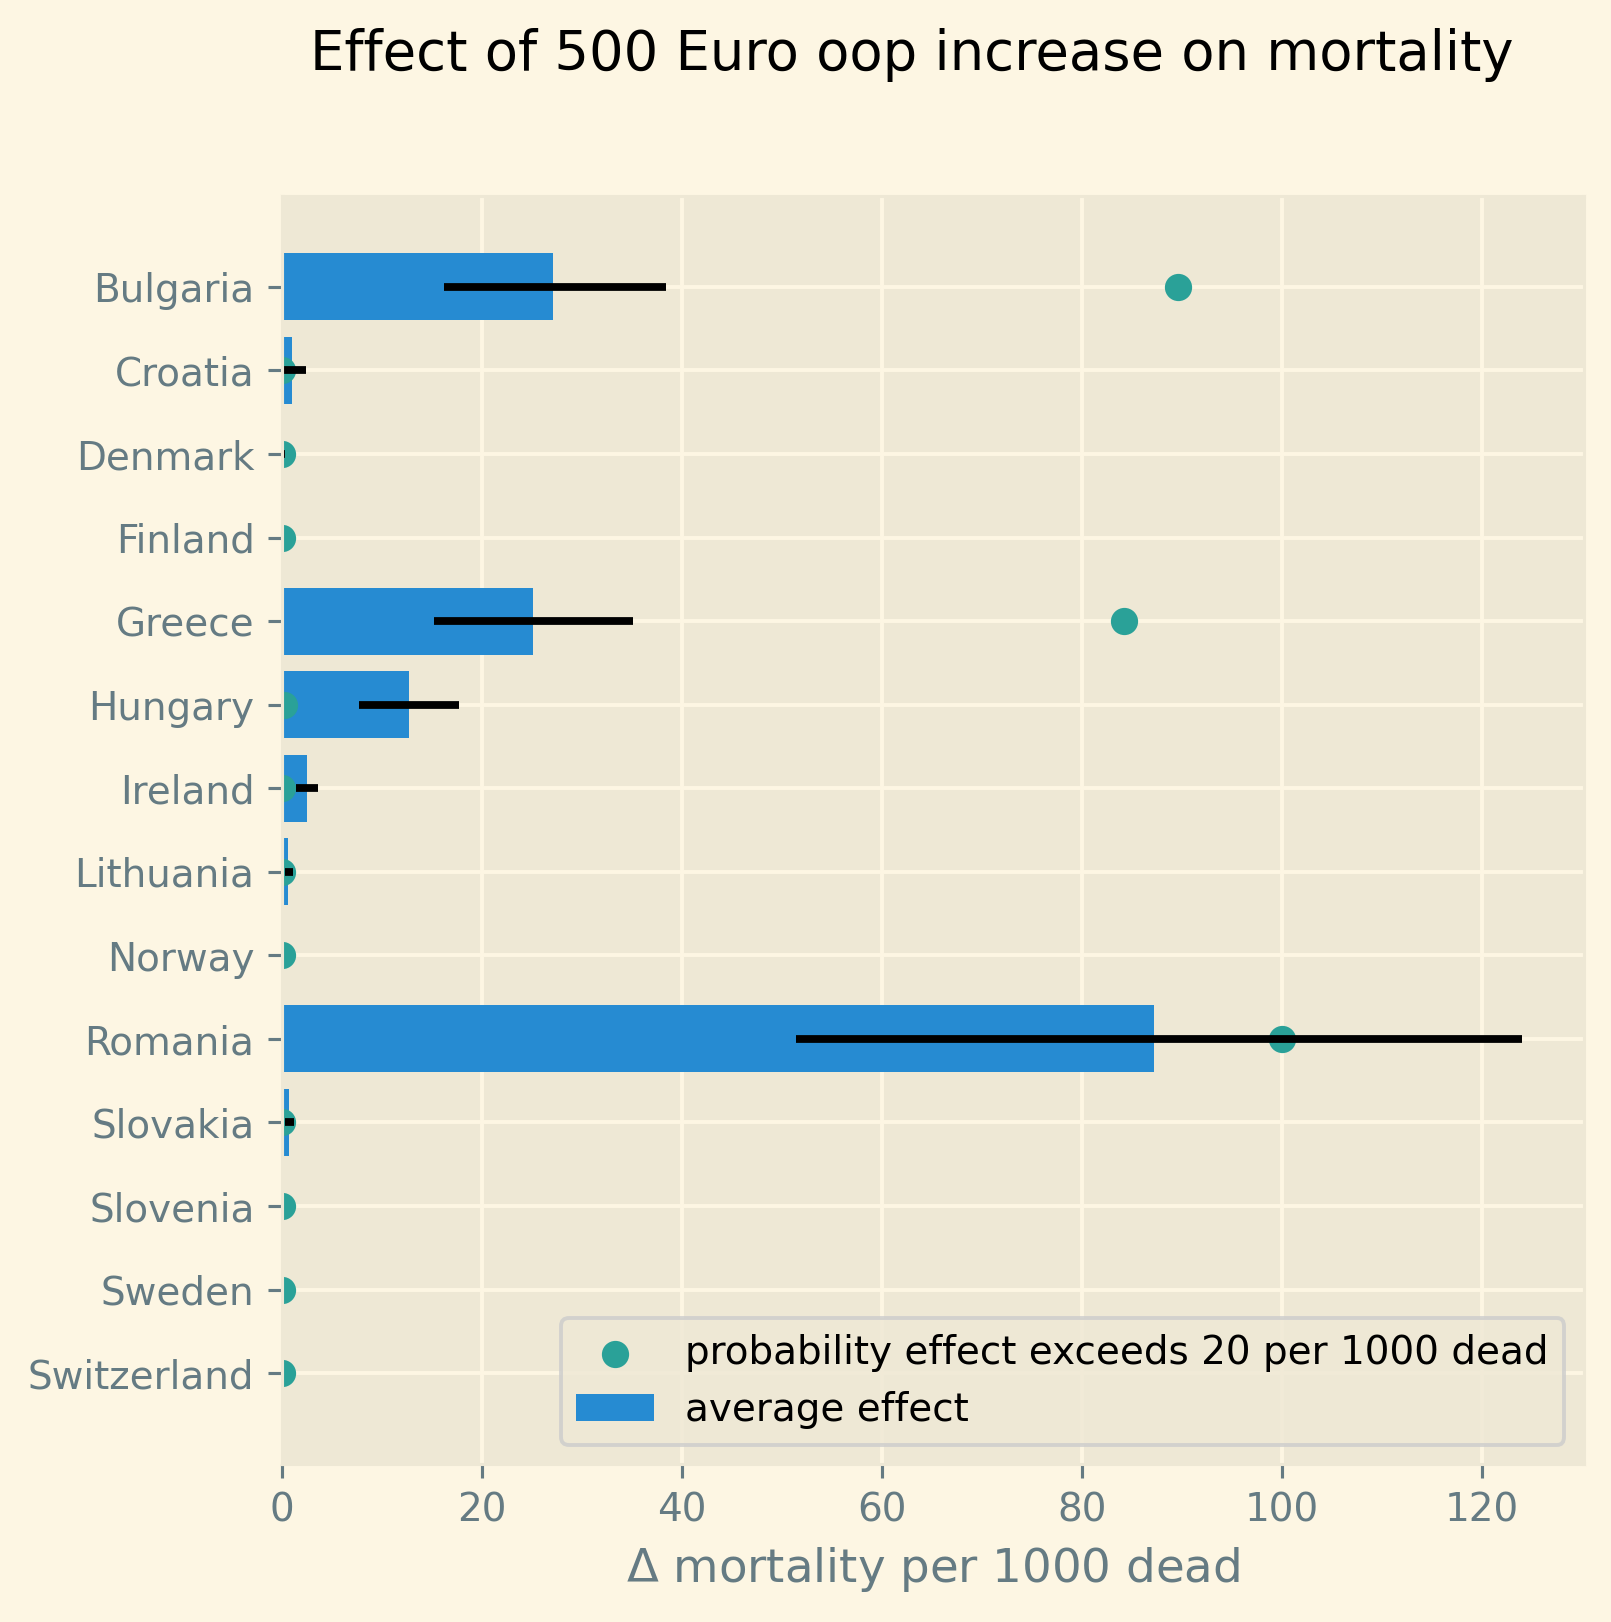
\includegraphics[width=0.6\linewidth]{./figures/change_mortality_countries_baseline.png}
\label{fig:SummaryFigure}
\end{center}
\end{frame}




\begin{frame}[label={sec:org371db78},fragile]{Robustness analysis}
 \begin{itemize}
\item include voluntary health insurance payments in \texttt{OOP} measure
\item at risk of poverty as poverty measure
\item separate effect of \texttt{TooExp} and other unmet medical needs on mortality
\end{itemize}
\end{frame}



\section*{Conclusions}
\label{sec:org2554fad}

\begin{frame}[label={sec:org9e7d816}]{Policy implications}
\begin{itemize}
\item increasing oop leads to more costs than just risk aversion
\item doing without oop is not an option:
\begin{itemize}
\item means tested oop
\item let copayments vary with cost effectiveness of treatments
\end{itemize}
\end{itemize}
\end{frame}
\end{document}